\newpage
\section{Trigonometry}

In this section, we will cover a variety of trigonometric functions and their properties.

\subsection{Trigonometric Functions}

\begin{itemize}

    \item \( \sin(x) = \frac{1}{\csc(x)} \)

    \item \( \cos(x) = \frac{1}{\sec(x)}\)

    \item \( \tan(x) = \frac{\sin(x)}{\cos(x)}\ = \frac{1}{\cot(x)}\)

    \item \( \csc(x) = \frac{1}{\sin(x)} \)

    \item \( \sec(x) = \frac{1}{\cos(x)} \)

    \item \( \cot(x) = \frac{\cos(x)}{\sin(x)} = \frac{1}{\tan(x)} \)

\end{itemize}

\subsection{SOH-CAH-TOA}

\begin{itemize}

    \item \( \sin(x) = \frac{\text{opposite}}{\text{hypotenuse}} \)

    \item \( \cos(x) = \frac{\text{adjacent}}{\text{hypotenuse}} \)

    \item \( \tan(x) = \frac{\text{opposite}}{\text{adjacent}} \)

\end{itemize}

\subsection{Pythagorean Identities}

\begin{itemize}

    \item \( \sin^2(x) + \cos^2(x) = 1 \)

    \item \( 1 + \tan^2(x) = \sec^2(x) \)

    \item \( 1 + \cot^2(x) = \csc^2(x) \)

\end{itemize}

\subsection{Sum and Difference Formulas}

\begin{itemize}

    \item \( \sin(a + b) = \sin(a)\cos(b) + \cos(a)\sin(b) \)

    \item \( \sin(a - b) = \sin(a)\cos(b) - \cos(a)\sin(b) \)

    \item \( \cos(a + b) = \cos(a)\cos(b) - \sin(a)\sin(b) \)

    \item \( \cos(a - b) = \cos(a)\cos(b) + \sin(a)\sin(b) \)

    \item \( \tan(a + b) = \frac{\tan(a) + \tan(b)}{1 - \tan(a)\tan(b)}\)

    \item \( \tan(a - b) = \frac{\tan(a) - \tan(b)}{1 + \tan(a)\tan(b)}\)
\end{itemize}

\begin{center}
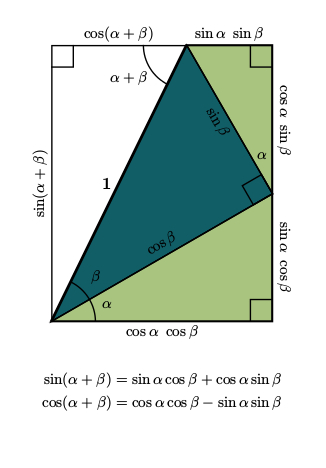
\includegraphics{trig.jpg}
\end{center}

\subsection{Double Angle Formulas}

\begin{itemize}

    \item \( \sin(2x) = 2\sin(x)\cos(x) \)

    \item \( \cos(2x) = \cos^2(x) - \sin^2(x) = 2\cos^2(x) - 1 = 1 - 2\sin^2(x) \)

    \item \( \tan(2x) = \frac{2\tan(x)}{1 - \tan^2(x)}\)

    \item \( \csc(2x) = \frac{2\csc(x)\sec(x)}{1 - \tan^2(x)}\)

    \item \( \sec(2x) = \frac{1 + \tan^2(x)}{2\tan(x)}\)

    \item \( \cot(2x) = \frac{1 - \tan^2(x)}{2\tan(x)}\)

\end{itemize}

\subsection{Half Angle Formulas}

\begin{itemize}

    \item \( \sin\left(\frac{x}{2}\right) = \pm\sqrt{\frac{1 - \cos(x)}{2}} \)

    \item \( \cos\left(\frac{x}{2}\right) = \pm\sqrt{\frac{1 + \cos(x)}{2}} \)

    \item \( \tan\left(\frac{x}{2}\right) = \frac{\sin(x)}{1 + \cos(x)} = \frac{1 - \cos(x)}{\sin(x)} = \frac{\tan(x)}{1 + \tan^2(x)}\)

    \item \( \csc\left(\frac{x}{2}\right) = \frac{1}{\sin\left(\frac{x}{2}\right)} = \pm\sqrt{\frac{2}{1 - \cos(x)}} \)

    \item \( \sec\left(\frac{x}{2}\right) = \frac{1}{\cos\left(\frac{x}{2}\right)} = \pm\sqrt{\frac{2}{1 + \cos(x)}} \)

    \item \( \cot\left(\frac{x}{2}\right) = \frac{1}{\tan\left(\frac{x}{2}\right)} = \frac{1 + \cos(x)}{\sin(x)} = \frac{1 - \tan^2(x)}{2\tan(x)}\)

\end{itemize}

\subsection{Product to Sum Formulas}

\begin{itemize}

    \item \( \sin(a)\sin(b) = \frac{1}{2}[\cos(a - b) - \cos(a + b)] \)

    \item \( \cos(a)\cos(b) = \frac{1}{2}[\cos(a - b) + \cos(a + b)] \)

    \item \( \sin(a)\cos(b) = \frac{1}{2}[\sin(a + b) + \sin(a - b)] \)

    \item \( \cos(a)\sin(b) = \frac{1}{2}[\sin(a + b) - \sin(a - b)] \)

\end{itemize}

\subsection{Power Reducing Formulas}

\begin{itemize}

    \item \( \sin^2(x) = \frac{1 - \cos(2x)}{2} \)

    \item \( \cos^2(x) = \frac{1 + \cos(2x)}{2} \)

    \item \( \tan^2(x) = \frac{1 - \cos(2x)}{1 + \cos(2x)}\)

    \item \( \csc^2(x) = \frac{1}{\sin^2(x)} = \frac{2}{1 - \cos(2x)} \)

    \item \( \sec^2(x) = \frac{1}{\cos^2(x)} = \frac{2}{1 + \cos(2x)} \)

    \item \( \cot^2(x) = \frac{1}{\tan^2(x)} = \frac{1 + \cos(2x)}{1 - \cos(2x)}\)

\end{itemize}

\subsection{Even and Odd Functions}

\begin{itemize}

    \item \( \sin(-x) = -\sin(x) \)

    \item \( \cos(-x) = \cos(x) \)

    \item \( \tan(-x) = -\tan(x) \)

    \item \( \csc(-x) = -\csc(x) \)

    \item \( \sec(-x) = \sec(x) \)

    \item \( \cot(-x) = -\cot(x) \)

\end{itemize}

\subsection{Graph Identity}

\(\cos(x) = \sin(x + \frac{\pi}{2})\)

\subsection{Trigonometric Values}
\smallskip

\begin{center}
    \renewcommand{\arraystretch}{1.4}
    \begin{tabular}{|c|c|c|c|}
    \hline
    \(\theta\) (radians) & \(\sin(\theta)\) & \(\cos(\theta)\) & \(\tan(\theta)\) \\
    \hline
    \(0\) & \(0\) & \(1\) & \(0\) \\
    \hline
    \(\frac{\pi}{6}\) & \(\frac{1}{2}\) & \(\frac{\sqrt{3}}{2}\) & \(\frac{1}{\sqrt{3}}\) \\
    \hline
    \(\frac{\pi}{4}\) & \(\frac{\sqrt{2}}{2}\) & \(\frac{\sqrt{2}}{2}\) & \(1\) \\
    \hline
    \(\frac{\pi}{3}\) & \(\frac{\sqrt{3}}{2}\) & \(\frac{1}{2}\) & \(\sqrt{3}\) \\
    \hline
    \(\frac{\pi}{2}\) & \(1\) & \(0\) & undefined \\
    \hline
    \(\frac{2\pi}{3}\) & \(\frac{\sqrt{3}}{2}\) & \(-\frac{1}{2}\) & \(-\sqrt{3}\) \\
    \hline
    \(\frac{3\pi}{4}\) & \(\frac{\sqrt{2}}{2}\) & \(-\frac{\sqrt{2}}{2}\) & \(-1\) \\
    \hline
    \(\frac{5\pi}{6}\) & \(\frac{1}{2}\) & \(-\frac{\sqrt{3}}{2}\) & \(-\frac{1}{\sqrt{3}}\) \\
    \hline
    \(\pi\) & \(0\) & \(-1\) & \(0\) \\
    \hline
    \(\frac{7\pi}{6}\) & \(-\frac{1}{2}\) & \(-\frac{\sqrt{3}}{2}\) & \(\frac{1}{\sqrt{3}}\) \\
    \hline
    \(\frac{5\pi}{4}\) & \(-\frac{\sqrt{2}}{2}\) & \(-\frac{\sqrt{2}}{2}\) & \(1\) \\
    \hline
    \(\frac{4\pi}{3}\) & \(-\frac{\sqrt{3}}{2}\) & \(-\frac{1}{2}\) & \(\sqrt{3}\) \\
    \hline
    \(\frac{3\pi}{2}\) & \(-1\) & \(0\) & undefined \\
    \hline
    \(\frac{5\pi}{3}\) & \(-\frac{\sqrt{3}}{2}\) & \(\frac{1}{2}\) & \(-\sqrt{3}\) \\
    \hline
    \(\frac{7\pi}{4}\) & \(-\frac{\sqrt{2}}{2}\) & \(\frac{\sqrt{2}}{2}\) & \(-1\) \\
    \hline
    \(\frac{11\pi}{6}\) & \(-\frac{1}{2}\) & \(\frac{\sqrt{3}}{2}\) & \(-\frac{1}{\sqrt{3}}\) \\
    \hline
    \(2\pi\) & \(0\) & \(1\) & \(0\) \\
    \hline
    \end{tabular}
\end{center}

\subsection{Unit Circle and Trigonometric Functions}

The unit circle is a circle with a radius of 1 centered at the origin. Trigonometric functions like \(\sin(\theta)\), \(\cos(\theta)\), and \(\tan(\theta)\) can be defined based on the coordinates of a point on the circle corresponding to angle \(\theta\).

\begin{center}
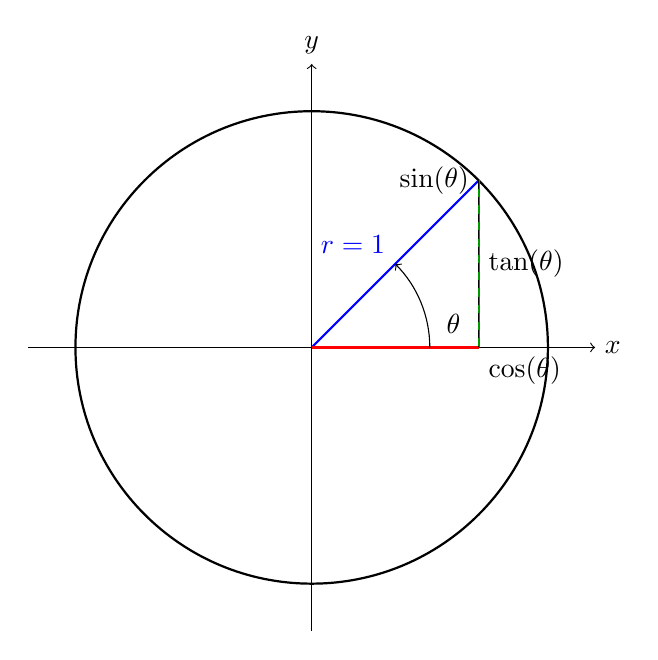
\begin{tikzpicture}[scale=3]
    % Draw unit circle
    \draw[thick] (0,0) circle (1);
    
    % Axes
    \draw[->] (-1.2,0) -- (1.2,0) node[right] {\(x\)};
    \draw[->] (0,-1.2) -- (0,1.2) node[above] {\(y\)};
    
    % Angle and triangle
    \draw[thick, blue] (0,0) -- ({cos(45)},{sin(45)}) node[pos=0.5, above left] {\(r=1\)};
    \draw[thick, red] (0,0) -- ({cos(45)},0);
    \draw[thick, green!60!black] ({cos(45)},0) -- ({cos(45)},{sin(45)});
    
    % Dotted lines
    \draw[dashed] ({cos(45)},{sin(45)}) -- ({cos(45)},0);
    
    % Angle arc
    \draw[->] (0.5,0) arc[start angle=0,end angle=45,radius=0.5];
    \node at (0.6,0.1) {\(\theta\)};
    
    % Labels
    \node[below right] at ({cos(45)},0) {\(\cos(\theta)\)};
    \node[left] at ({cos(45)},{sin(45)}) {\(\sin(\theta)\)};
    \node[right] at ({cos(45)}, {sin(45)/2}) {\(\tan(\theta)\)};
\end{tikzpicture}
\end{center}

\subsection{Definitions on the Unit Circle:}

\begin{itemize}

    \item \(\cos(\theta)\) is the \emph{x-coordinate} of the point on the circle.

    \item \(\sin(\theta)\) is the \emph{y-coordinate}.

    \item \(\tan(\theta) = \dfrac{\sin(\theta)}{\cos(\theta)}\) is the ratio of the opposite side to the adjacent side in the triangle.

\end{itemize}


\subsection{Trigonometric Rules}

\begin{itemize}[label =\(-\)]

    \item \(\frac{\sin \alpha}{a} = \frac{\sin \beta}{b} = \frac{\sin \gamma}{c}\)

    \item \(c^2 = a^2 + b^2 - 2ab \cos \gamma\)

    \item \(\frac{a - b}{a + b} = \frac{\tan \frac{1}{2}(\alpha - \beta)}{\tan \frac{1}{2} (\alpha + \beta)}\)

\end{itemize}


\subsection{Proof of the Cosine Rule}

The \emph{Cosine Rule} relates the lengths of the sides of a triangle to the cosine of one of its angles. 
For any triangle \( ABC \) with sides \( a = BC \), \( b = AC \), and \( c = AB \), and angle 
\( \gamma = \angle ACB \), the cosine rule states:

\[
    c^2 = a^2 + b^2 - 2ab\cos(\gamma)
\]

\textbf{Proof}

Consider triangle \( ABC \), and place it on the coordinate plane such that point \( C \) is at the origin
\( (0,0) \), point \( B \) is at \( (a,0) \), and point \( A \) lies somewhere in the plane. 
Let angle \( \gamma = \angle ACB \).
\vspace{\baselineskip}

Let the coordinates of point \( A \) be \( (b\cos\gamma, b\sin\gamma) \), since \( b = AC \) and we’re 
using polar coordinates to define its location relative to point \( C \).
\vspace{\baselineskip}

Using the distance formula to find side \( c = AB \), we get:

\begin{align*}
    c^2 &= {(a - b\cos\gamma)}^2 + {(0 - b\sin\gamma)}^2 \\
    &= a^2 - 2ab\cos\gamma + b^2\cos^2\gamma + b^2\sin^2\gamma \\
    &= a^2 + b^2(\cos^2\gamma + \sin^2\gamma) - 2ab\cos\gamma \\
    &= a^2 + b^2 - 2ab\cos\gamma
\end{align*}

Since \( \cos^2\gamma + \sin^2\gamma = 1 \).
\vspace{\baselineskip}

Thus, we have proven that:

\[
    c^2 = a^2 + b^2 - 2ab\cos\gamma
\]

\QED